\documentclass{article}

\usepackage{graphicx}
\usepackage{tikz}
\usepackage{tikzsymbols}
\usetikzlibrary{calc,patterns,shapes.geometric}
\pagestyle{empty}
\usepackage[margin=0pt]{geometry}
\geometry{papersize={14in,12in}}

\def\centerarc[#1](#2)(#3:#4:#5){\draw[#1] ($(#2)+({#5*cos(#3)},{#5*sin(#3)})$) arc (#3:#4:#5);}

\begin{document}
	\begin{figure}
		\centering
		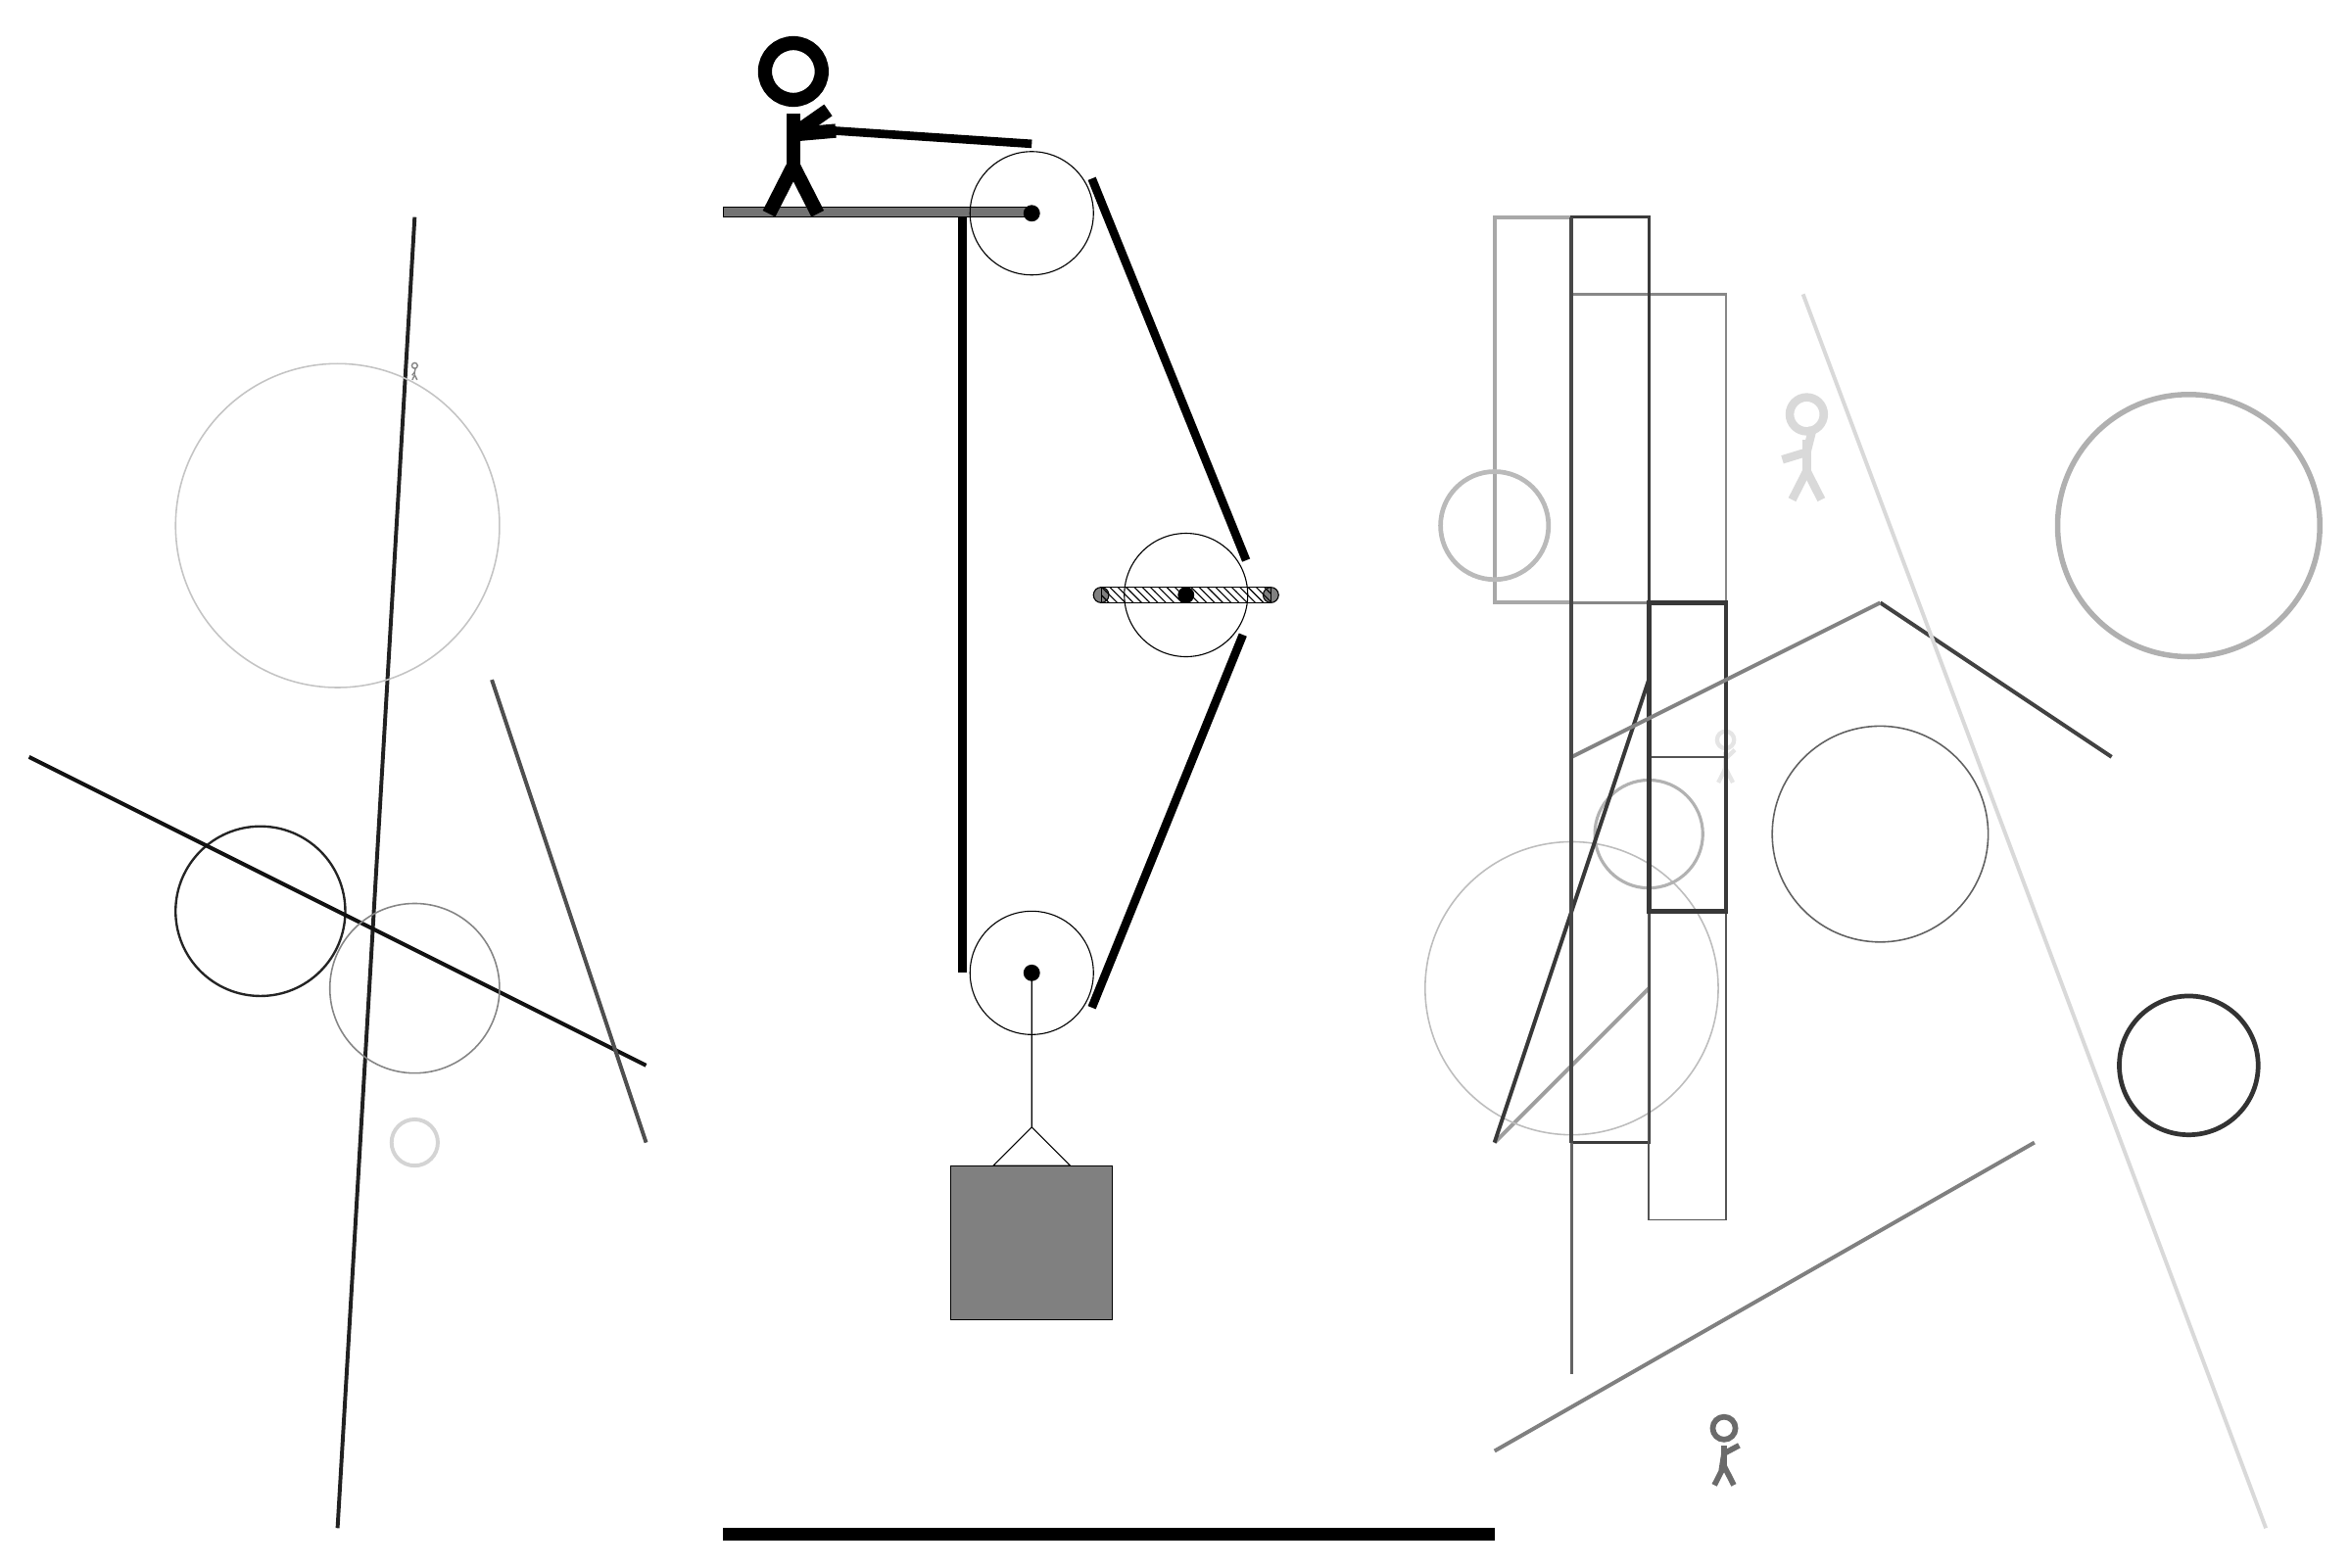
\begin{tikzpicture}
			%%%%% START %%%%%
			
			\draw[fill=black!55] (-2, 14) rectangle (2, 14.125);
			
			\draw (2, 4.2) circle (0.8);
			\draw[fill=black] (2, 4.2) circle (0.1);
			
			\draw (2, 14.05) circle (0.8);
			\draw[fill=black] (2, 14.05) circle (0.1);
			
			\draw[fill=white](4, 9.1) circle (0.8);
			\draw[fill=black] (4, 9.1) circle (0.1);
			\draw[fill=black!50] (2.9, 9.1) circle (0.1);
			\draw[fill=black!50] (5.1, 9.1) circle (0.1);
			\draw[pattern=north west lines, pattern color=black] (2.9, 9.2) rectangle (5.1, 9.0);
			
			\draw (2, 4.2) -- (2, 2.2) -- (1.5, 1.7) -- (2.5, 1.7) -- (2, 2.2);
			\draw[fill=black!50] (0.95, 1.7) rectangle (3.05, -0.3);
			
			\draw[line width=1.1mm] (1.1, 14) -- (1.1, 4.2);
			\centerarc[line width=1.1mm](2, 4.2)(180:330:0.9);
			\draw[line width=1.1mm](2.7794, 3.75) -- (4.7373, 8.5838);
			\centerarc[line width=1.1mm](4, 9.1)(390:325:0.9);
			\draw[line width=1.1mm](4.7794, 9.55) -- (2.7794, 14.5);
			\centerarc[line width=1.1mm](2, 14.05)(30:90:0.9);
			\draw[line width=1.1mm](2, 14.95) -- (-1, 15.15);
			
			\node at (-1, 15.15) {\Strichmaxerl[10][-175][35]};
			
			\draw [line width=0.3mm, color=black!86](-8, 5) circle (1.1);
			
			\draw[line width=0.5mm, color=black!34] (8, 14) rectangle (9, 9);
			\draw[line width=0.5mm, color=black!38](10, 4) -- (8, 2);
			\node[line width=0.3mm, color=black!10] at (11, 7) {\Strichmaxerl[3][86][44]};
			
			\draw[line width=0.3mm, color=black!47] (9, 13) rectangle (11, 9);
			
			\draw[line width=0.5mm, color=black!87](-7, -3) -- (-6, 14);
			
			\draw [line width=0.2mm, color=black!26](9, 4) circle (1.9);
			\draw[line width=0.5mm, color=black!50](8, -2) -- (15, 2);
			\draw[line width=0.5mm, color=black!93](-3, 3) -- (-11, 7);
			
			\draw[line width=0.4mm, color=black!77] (9, 14) rectangle (10, 2);
			\draw[line width=0.5mm, color=black!74](13, 9) -- (16, 7);
			
			\draw [line width=0.6mm, color=black!27](8, 10) circle (0.7);
			\draw [line width=0.7mm, color=black!31](17, 10) circle (1.7);
			
			\node[line width=0.6mm, color=black!47] at (-6, 12) {\Strichmaxerl[1][54][79]};
			\draw [line width=0.2mm, color=black!23](-7, 10) circle (2.1);
			\draw[line width=0.5mm, color=black!15](12, 13) -- (18, -3);
			
			\draw [line width=0.2mm, color=black!62](13, 6) circle (1.4);
			\draw [line width=0.5mm, color=black!17](-6, 2) circle (0.3);
			\draw [line width=0.4mm, color=black!30](10, 6) circle (0.7);
			
			\draw [line width=0.6mm, color=black!80](17, 3) circle (0.9);
			\node[line width=0.4mm, color=black!58] at (11, -2) {\Strichmaxerl[4][81][28]};
			
			\node[line width=0.4mm, color=black!15] at (12, 11) {\Strichmaxerl[6][17][76]};
			
			\draw [line width=0.2mm, color=black!48](-6, 4) circle (1.1);
			\draw[line width=0.5mm, color=black!69](-3, 2) -- (-5, 8);
			\draw[line width=0.2mm, color=black!67] (10, 1) rectangle (11, 7);
			
			\draw[line width=0.6mm, color=black!78] (10, 9) rectangle (11, 5);
			
			\draw[line width=0.3mm, color=black!61] (9, -1) rectangle (9, 2);
			\draw[line width=0.5mm, color=black!78](10, 8) -- (8, 2);
			\draw[line width=0.5mm, color=black!49](13, 9) -- (9, 7);
			\draw[line width=0.5mm, color=black!72](9, 2) -- (9, 14);
			
			\draw[fill=black] (-2, -3) rectangle (8, -3.15);
			
			%%%%% END %%%%%
		\end{tikzpicture}
	\end{figure}	
\end{document}